\section{The System\label{sec:system}}

% High-level architecture

\begin{figure}
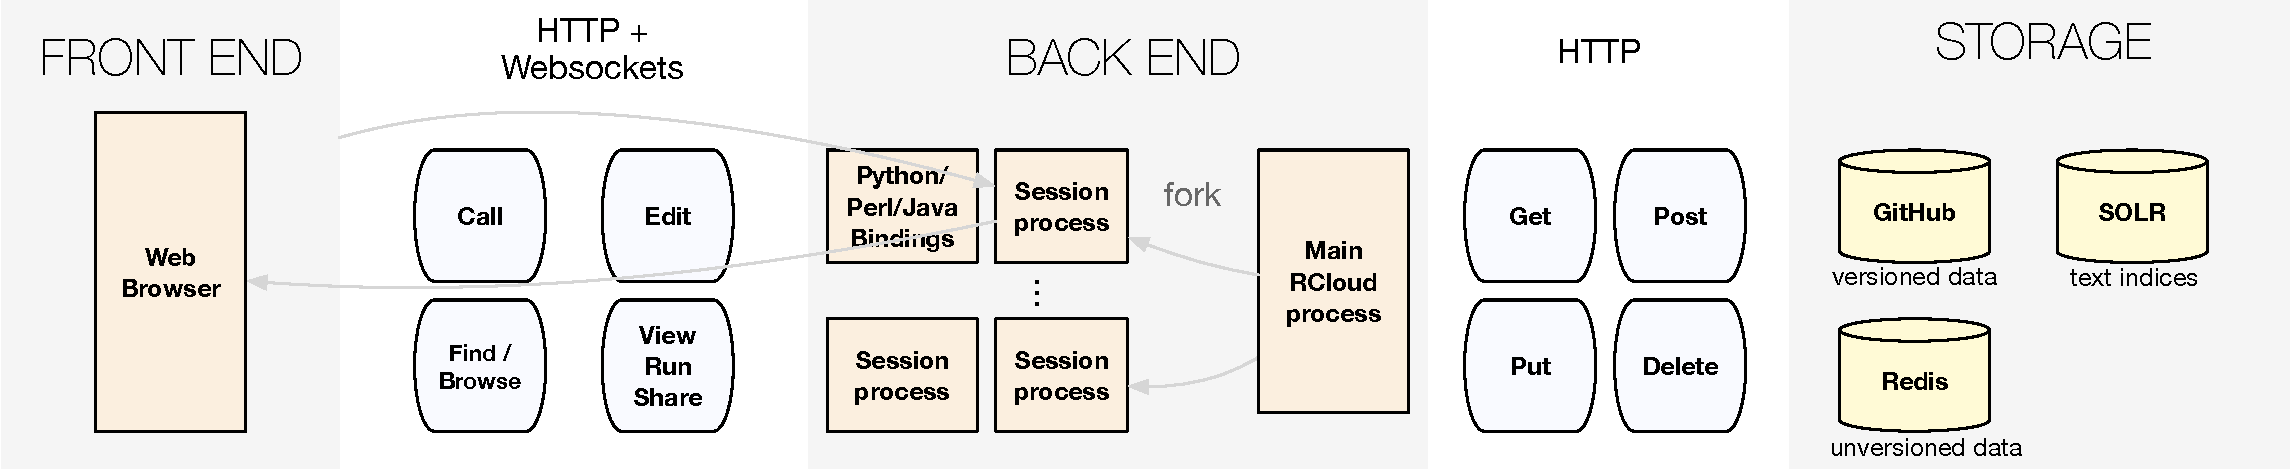
\includegraphics[width=\linewidth]{fig/system/system.pdf}
\caption{\label{fig:system}A diagram of RCloud's architecture. Dashed
  lines represent features which not yet implemented.}
\end{figure}

The internal computing infrastructure of organizations has changed
radically in the last fifteen years. The shift from large
servers toward scalable, lower-cost, distributed systems (``the cloud'')
led to a software ecosystem of processes distributed over a
network (often virtually defined) communicating via some
high-level protocol, usually HTTP.  HTTP is dominant because web
browsers and servers are ubiquitous and available in almost
all hardware devices, from tiny sensors, to handheld devices and
laptops, to rack-mounted servers.

As a result, HTTP is the lingua franca of interprocess communication
(IPC). One of the design goals for RCloud was to provide an attractive
environment for creators of data-analysis scripts, that also behaves
as a first-class citizen in the pre-existing ecosystem of computer
services and networks with an organization.

%% Design for cloud-friendly? This goes back to the point in the
%% introduction about playing nice with the rest of the ecosystem.

\subsection{System Design}

We designed RCloud around the front-facing API, which provides roughly
one entry point to correspond with each requirement.

Edit

View/Run/Share

Call

Browse/Search. ``More like this'', and a custom webpage solely for browsing.

\subsection{Notebooks\label{sec:notebooks}}

\begin{figure*}
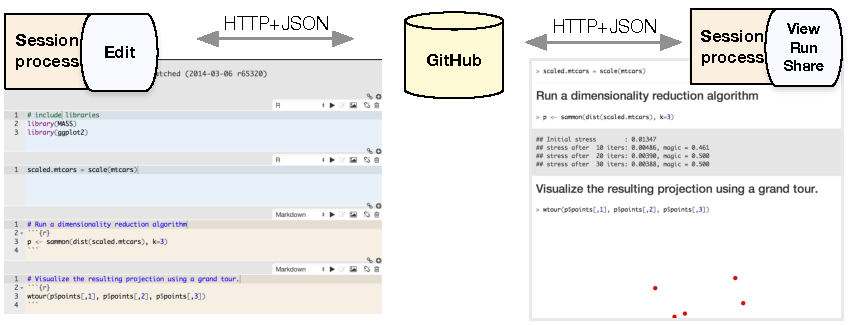
\includegraphics[width=\linewidth]{fig/notebook/notebook.pdf}
\caption{\label{fig:notebook}An RCloud notebook is a sequence of
  \emph{cells}, each a snippet of source in R or Markdown. Notebooks
  are stored in GitHub \emph{gists}, which provide the version-control
  primitives needed in RCloud during editing (left) or viewing and
  executing (right).}
\end{figure*}

The basic unit of operation in RCloud is a \emph{notebook}. RCloud
notebooks hold a sequence of \emph{cells}, each of which represents a
snippet of code or hypertext in Markdown. This is not a novel idea;
executable documents structured in this way are present in a wide
variety of present software systems, from Mathematica to IPython to
Sage and others.

One of the main differences between RCloud and other systems is the
notion that notebooks are ``always deployed''. This has a variety of
advantages which we discuss \todo{where?}. On the other hand, there
are a variety of situations that might ask for a specific version of a
notebook. Rather than have the notebook designer decide ahead of time
which versions should be preserved, we choose to expose
\emph{transparent} versioning. This is similar to models like
Jankun-Kelly et al.'s p-set calculus \todo{cite} and VisTrails's
version tree \todo{cite}, where every change in the state of the
system is tracked.

Implementing the entire version-control subsystem would be a large
undertaking. Instead, we build the infrastructure on top of Github's
\emph{gists}~\todo{cite}. Github offers a HTTP interface
for creating simplified git repositories (the main limitation is the
use of text-only files and a single directory). The GitHub web-service
API provides much of the infrastructure we need for the versioning
portion of the storage back end: access to previous versions,
comments, starring, and forking.

Using GitHub was mainly a tactical decision to reduce our
time-to-prototype. At the same time, it had the fortuitous decision of
forcing our backend to communicate with separate processes over HTTP
and JSON. This had the serendipitous advantage of quickly enabling
full search over RCloud notebooks (built using Apache SOLR).
%
This perspective has implications for
systems-based research and prototyping in visual analytics.
%
In order for small teams to efficiently explore ideas in the present
software ecosystem, it pays off to use as many existing solutions as
possible.
%
Even though it involved learning a variety of standards that are not
directly related to visual analytics, our early decision to use the
GitHub gist API has been quite fruitful. We expect similar payoffs to
happen for related projects as well.

%% %
%% We needed version control over a directory, gist provides that,
%% wrapped over an HTTP interface.
%% %
%% Mainly a tactical decision to save time.
%% %
%% Nevertheless, availability of notebook data as (barely) plain text had good side
%% effects, like ease to build search.
%% %
%% Expect same with suggest.

\subsection{Reputation and Interest: starring\label{sec:starring}}

In RCloud, reputation and interest are a relationship between
\emph{notebooks} and \emph{users}, rather than a relationship between
user pairs. We decided on this approach because we expect typical
RCloud deployments to have relatively few users, but each user to have
written relatively many notebooks. Under that assumption, assigning
interest to users would not provide sufficiently ``high-resolution'' data.

We incorporate both explicit and implicit indications of interest
in notebooks. Explicit interest is signaled by ``starring,'' or
clicking on a button that marks a notebook as interesting.
This makes explicit indication of interest a nearly trivial operation,
always readily available, thus encouraging its use.

Implicit signaling of interest is supported by keeping click-through
\cite{Joachims:2005:AIC} and execution counts. (In addition to these
classic techniques of collecting feedback from web search, we anticipate
applying static and dynamic code analysis to generate fine-grained
information about relationships, for example, which packages and data
sets often appear together.)

\subsection{Executing R in a web browser}

One our main goals is to provide ubiquitous access to the statistical
tools of the R programming language in the wider environment in which data
science teams participate.
%
Given the recent developments of interactive visualization and visual
analytics in HTML5 and the web, we decided to create an
\emph{interconnect} between the two environments.
%
Every RCloud session spawns a new R execution process in a remote
server. The communication between the web browser and the 

%% \subsubsection{Object capabilities: R to Javascript RPC and access
%%   control}

HTTP and web services are convenient but much of the protocol is
stateless. (For example, GET requests are required to not change the
remote state, and results can be cached in transparent proxies along
the network). In the case of close communication between a running
R process and a web browser, we seek something that is more flexible
than distinct URLs for every R process (with the resulting
complication in providing access 


%% \subsection{Technologies: R, Python, HTML5, interactive notebooks, etc.}

%% How do we do things that are not trivial to do with IPython (for
%% example)

%% What is relationship to a standard CMS with R/Python

%% dcplot. two-way communication between between backend session and
%% frontend session.

%% A key engineering decision in RCloud was to rely on full two-way
%% communication between the web client human interface, and data and
%% computing resources in the cloud. It is easier to engineer a design
%% in which the human interface is pushed one-way from the server
%% and thereafter all interaction takes place within the client.
%% Two-way communication is necessary, though, where the size of
%% the data or computational performance makes it impractical to
%% move all computation to the client.


\subsection{Deployment of notebooks\label{sec:deployment}}

Notebooks as versioned subroutines, web services.

There exists a URL for every notebook in RCloud, and notebooks by
default are visible by the entire organization. This is deliberate.
As pointed out by Wattenberg and Kriss~\cite{Wattenberg:2011:DFS},
broad access to analysis outputs (in their case, for NameVoyager)
increases long-term engagement in part through cross-references on
the web. Although our prototype RCloud deployment is only visible
inside a corporate intranet, we nevertheless found anecdotal support
for this notion by discovering links to RCloud notebooks in internal
discussion fora and mailing lists.
